

\section{User Module Sub-system}

\subsection{External Interfaces}
This section gives a detailed description of the system interfaces, hardware interfaces, software interfaces as well as communication interfaces.

	\subsubsection{System Interfaces}
		\begin{itemize}
			\item The user module will interface with any subsystem or module that wishes to access the data or functions.  
			
			\item 
		\end{itemize}
	\subsubsection{User Interfaces }
	\subsubsection{Hardware Interfaces }
	\subsubsection{Software Interfaces } %
	\subsubsection{Communication Interfaces } %
	
\subsection{Performance Requirements} %


\subsection{Design Constraints}



\subsection{Software System Attributes} %


\section{UML}
\subsection{Class Diagram}
The class diagram of the user sub-system makes use of the template method so that if need be one can easily construct different types of users with minimal code modifications.


\begin{figure}[H]
	\centering
	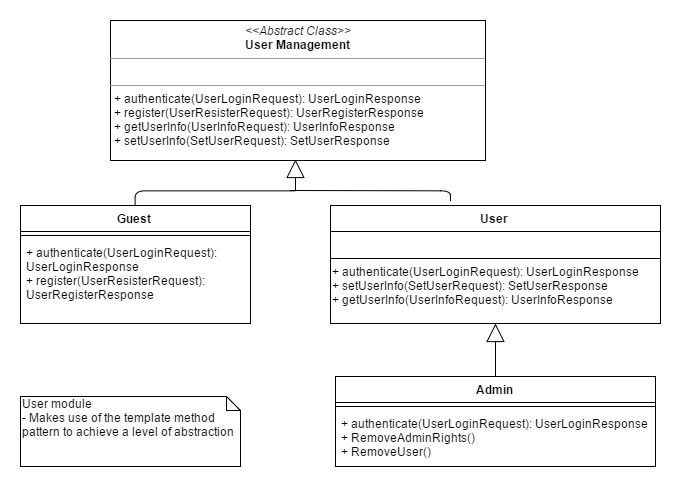
\includegraphics[width=0.7\textwidth]{user/img/UserClassDiagram.jpg}
	\caption{User Class Diagram}
\end{figure}



%\subsection{Deployment Diagram}
%
%\begin{figure}[H]
%%	\centering
%%	\includegraphics[width=\textwidth]{user/img/}
%%	\caption{}
%\end{figure}
%
%
\subsection{Activity Diagram}

\begin{figure}[H]
		\centering
		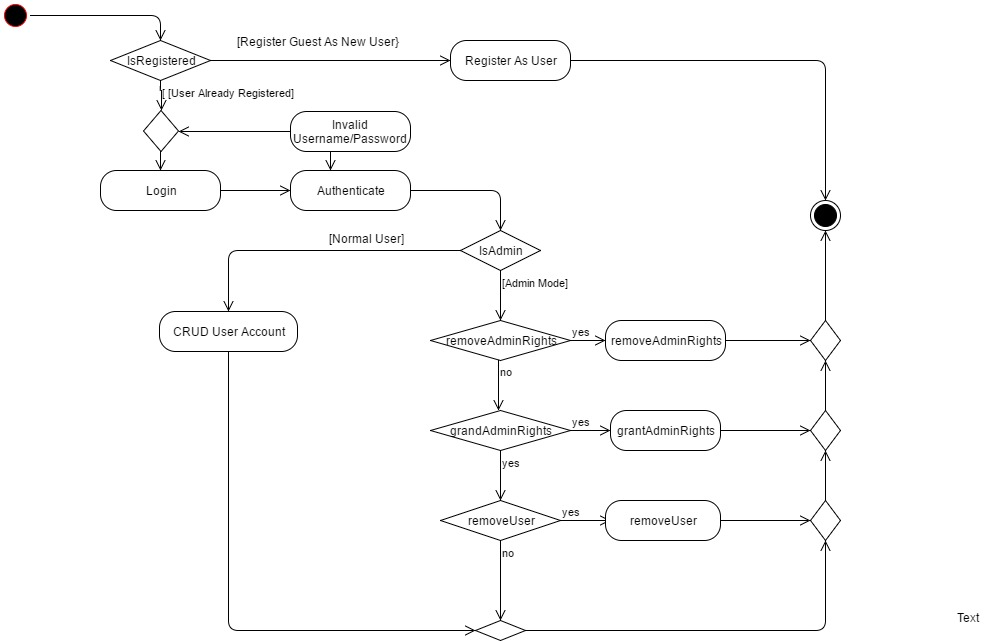
\includegraphics[width=\textwidth]{user/img/UserActivityDiagram.jpg}
		\caption{User Activity Diagram}
\end{figure}


\subsection{Sequence Diagram}

\begin{figure}[H]
		\centering
		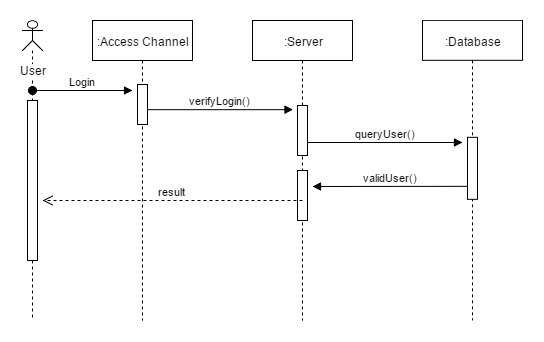
\includegraphics[width=0.7\textwidth]{user/img/UserSequence.jpg}
		\caption{User Login}
\end{figure}



\subsection{State Diagram}

\begin{figure}[H]
		\centering
		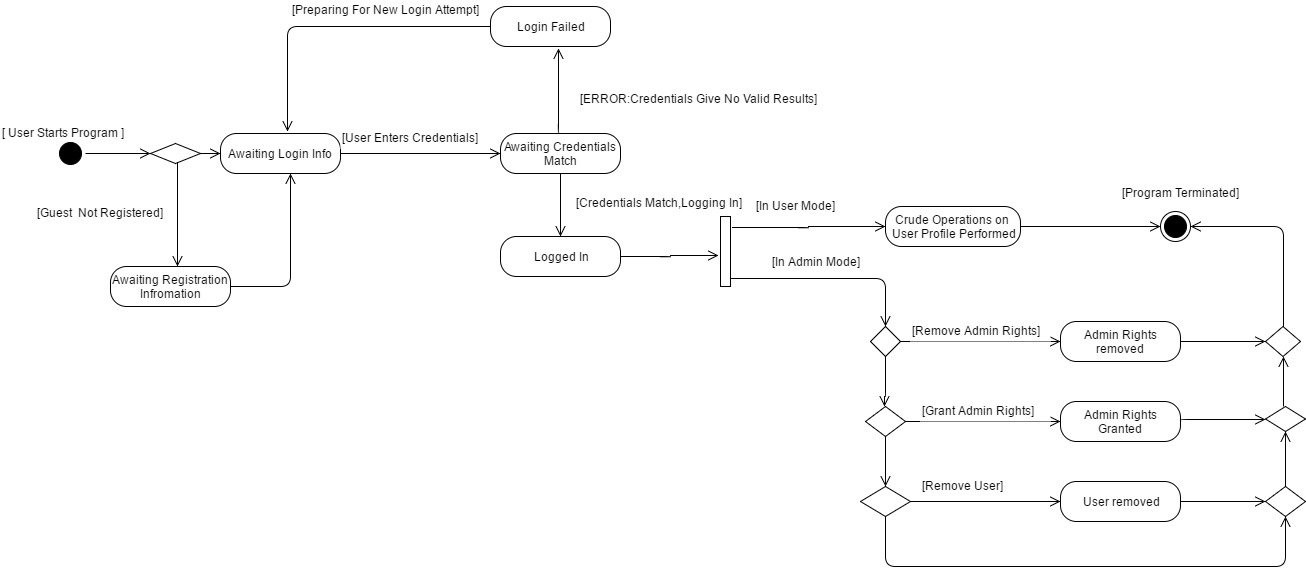
\includegraphics[width=\textwidth]{user/img/UserStateDiagram.jpg}
		\caption{User Login State Diagram}
\end{figure}




\subsection{Use Case Diagram}

\begin{figure}[H]
		\centering
		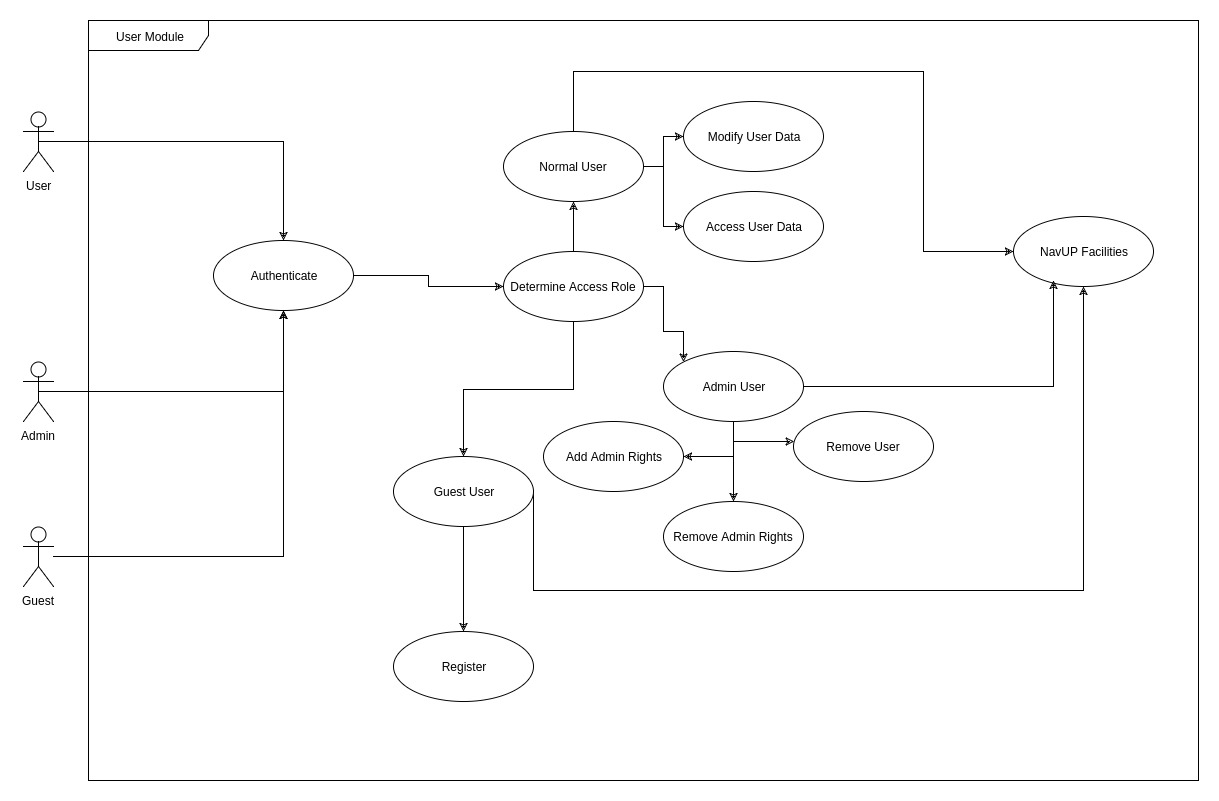
\includegraphics[width=0.7\textwidth]{user/img/UserUseCase.jpg}
		\caption{User Login with core functionality }
\end{figure}



